\documentclass[11pt]{article}
\usepackage{tikz}
\usepackage{amssymb}
\usepackage{geometry}
\geometry{letterpaper, landscape, margin=0.4in}
\usetikzlibrary{positioning, calc}

% Door macros
\newcommand{\hdoor}[2]{%
  \fill[white,draw=black,thick] ({#1-0.1},{#2-0.12}) rectangle ({#1+0.1},{#2+0.12});%
}
\newcommand{\vdoor}[2]{%
  \fill[white,draw=black,thick] ({#1-0.12},{#2-0.1}) rectangle ({#1+0.12},{#2+0.1});%
}

\begin{document}

\begin{center}
{\Huge \textbf{The Grain Mother's Ruin}}\\[0.3em]
{\Large Level 4 --- The Sealed Depths | 10 Keyed Areas}
\end{center}

\vspace{0.3em}

\begin{center}
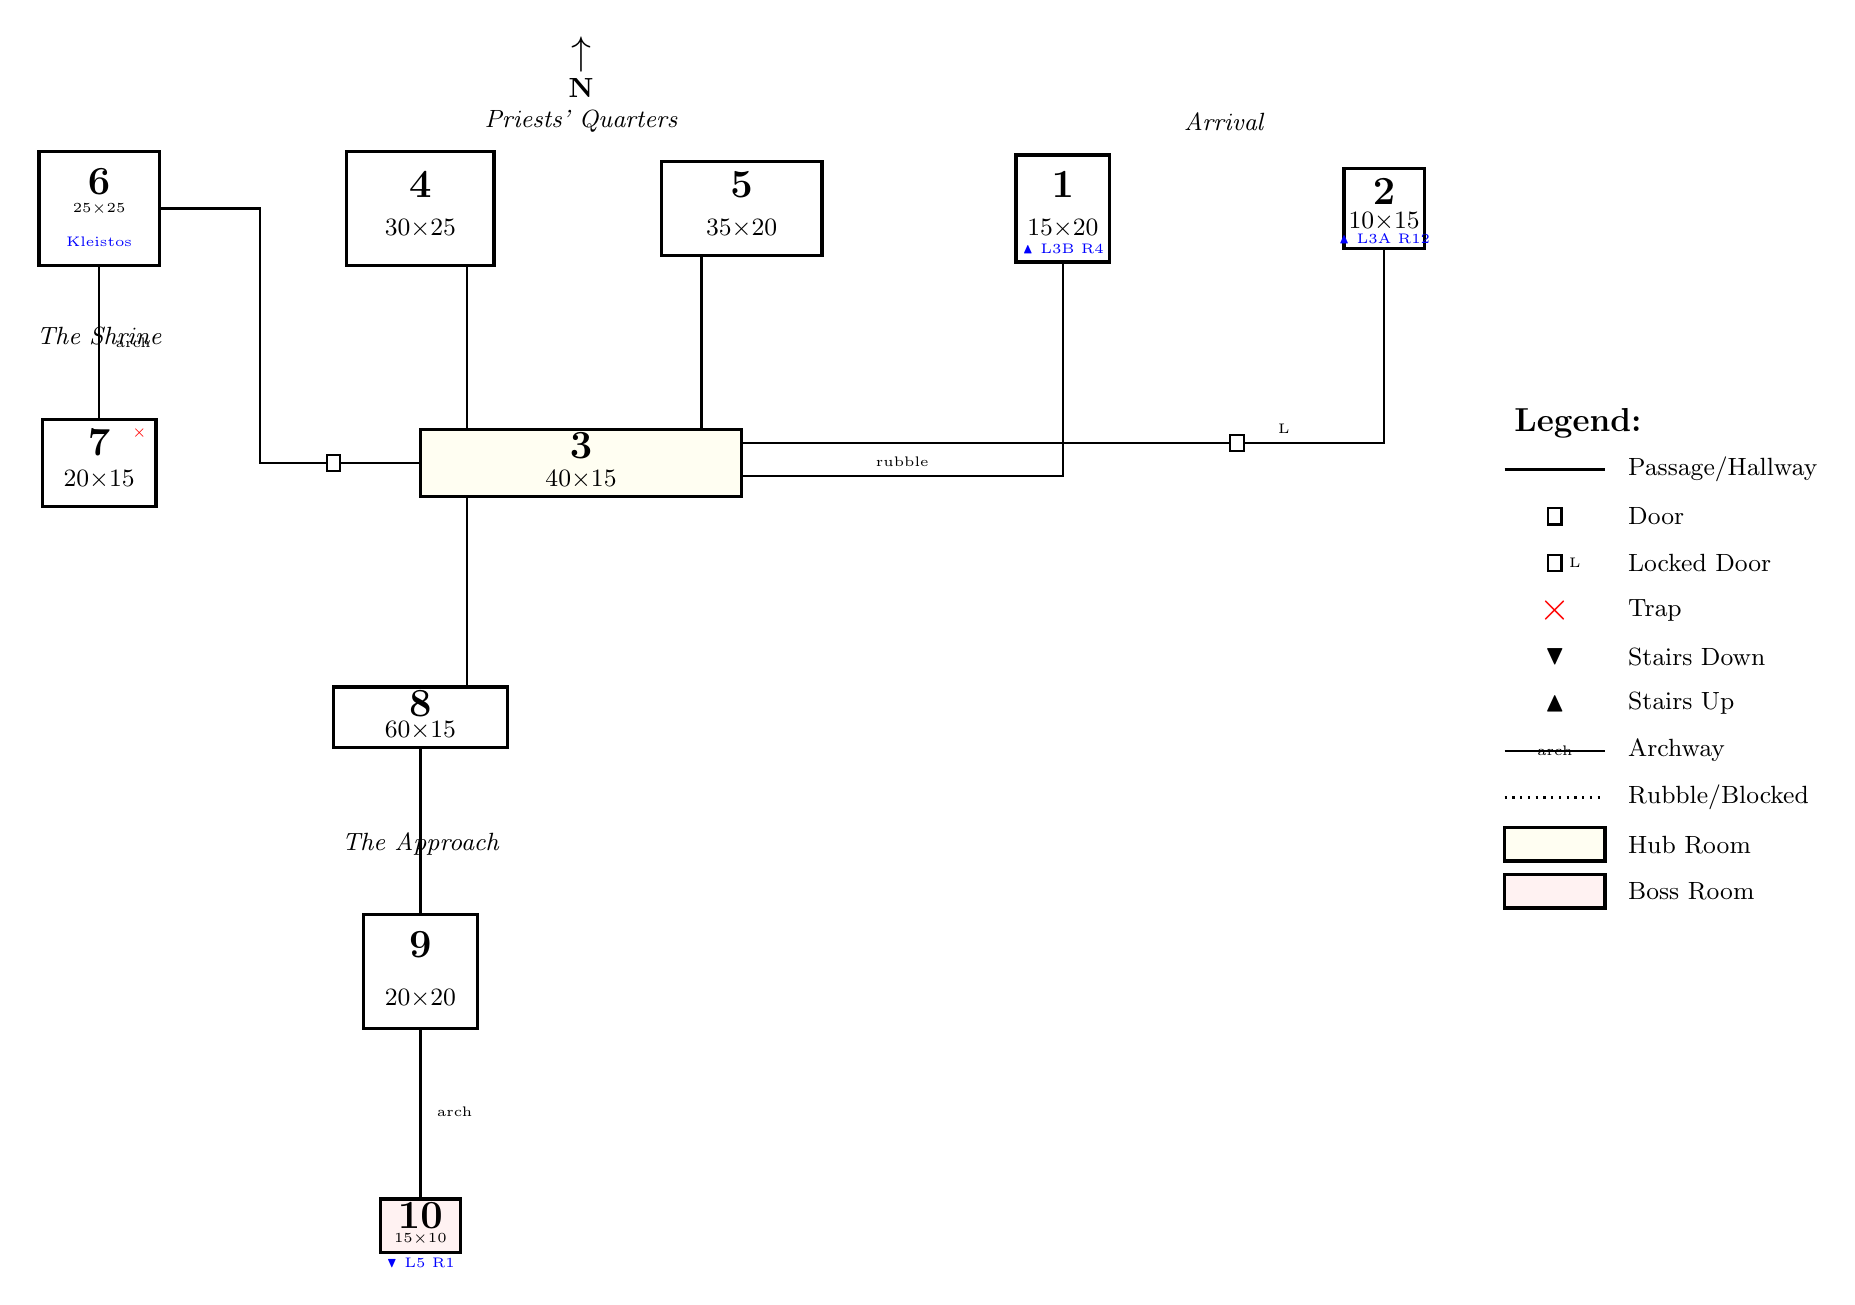
\begin{tikzpicture}[
    room/.style={draw, very thick, rectangle},
    hub/.style={draw, very thick, rectangle, fill=yellow!5},
    boss/.style={draw, very thick, rectangle, fill=red!5},
    connection/.style={draw, thick},
    secret/.style={dashed, thick},
    trap/.style={red},
    scale=0.85
]

% ============================================================
% GRID PARAMETERS
% CellW=3.0, CellH=2.0, Gutter=1.8
% Cols: c0(x=1.5) c1(x=6.3) c2(x=11.1) c3(x=15.9) c4(x=20.7)
% Rows: r0(y=1.0) r1(y=4.8) r2(y=8.6) r3(y=12.4) r4(y=16.2)
% Vertical gutters: c0-c1(x=3.9) c1-c2(x=8.7) c2-c3(x=13.5) c3-c4(x=18.3)
% Horizontal gutters: r0-r1(y=2.9) r1-r2(y=6.7) r2-r3(y=10.5) r3-r4(y=14.3)
% ============================================================

% ============================================================
% NORTH ARROW
% ============================================================
\node at (8.7, 18.5) {\Large $\uparrow$};
\node at (8.7, 18.0) {\textbf{N}};

% ============================================================
% ZONE: Arrival (Rooms 1-3)
% ============================================================

% Room 1: The Frozen Stair (15x20 ft, irregular)
% Cell: (c3, r4) -> center (15.9, 16.2)
% Rect: (15.2, 15.4) to (16.6, 17.0)
\draw[room] (15.2,15.4) rectangle (16.6,17.0);
\node at (15.9,16.55) {\Large \textbf{1}};
\node[font=\small] at (15.9,15.9) {15$\times$20};
\node[blue,font=\tiny] at (15.9,15.6) {$\blacktriangle$ L3B R4};

% Room 2: The Priest's Landing (10x15 ft)
% Cell: (c4, r4) -> center (20.7, 16.2)
% Rect: (20.1, 15.6) to (21.3, 16.8)
\draw[room] (20.1,15.6) rectangle (21.3,16.8);
\node at (20.7,16.45) {\Large \textbf{2}};
\node[font=\small] at (20.7,16.0) {10$\times$15};
\node[blue,font=\tiny] at (20.7,15.75) {$\blacktriangle$ L3A R12};

% Room 3: The Junction Hall (40x15 ft) -- HUB: 6 connections
% Cell: (c1-c2, r3) -> center (8.7, 12.4), spans 2 cells
% Rect: (6.3, 11.9) to (11.1, 12.9)
\draw[hub] (6.3,11.9) rectangle (11.1,12.9);
\node at (8.7,12.65) {\Large \textbf{3}};
\node[font=\small] at (8.7,12.15) {40$\times$15};

% ============================================================
% ZONE: The Priests' Quarters (Rooms 4-5)
% ============================================================

% Room 4: The Dormitory of the Faithful (30x25 ft)
% Cell: (c1, r4) -> center (6.3, 16.2)
% Rect: (5.2, 15.35) to (7.4, 17.05)
\draw[room] (5.2,15.35) rectangle (7.4,17.05);
\node at (6.3,16.55) {\Large \textbf{4}};
\node[font=\small] at (6.3,15.9) {30$\times$25};

% Room 5: The Refectory (35x20 ft)
% Cell: (c2, r4) -> center (11.1, 16.2)
% Rect: (9.9, 15.5) to (12.3, 16.9)
\draw[room] (9.9,15.5) rectangle (12.3,16.9);
\node at (11.1,16.55) {\Large \textbf{5}};
\node[font=\small] at (11.1,15.9) {35$\times$20};

% ============================================================
% ZONE: The Shrine (Rooms 6-7)
% ============================================================

% Room 6: The Shrine of Archon Kleistos (25x25 ft, domed)
% Cell: (c0, r4) -> center (1.5, 16.2)
% Rect: (0.6, 15.35) to (2.4, 17.05)
\draw[room] (0.6,15.35) rectangle (2.4,17.05);
\node at (1.5,16.6) {\Large \textbf{6}};
\node[font=\tiny] at (1.5,16.2) {25$\times$25};
\node[blue,font=\tiny] at (1.5,15.7) {Kleistos};

% Room 7: The Ritual Vestry (20x15 ft)
% Cell: (c0, r3) -> center (1.5, 12.4)
% Rect: (0.65, 11.75) to (2.35, 13.05)
\draw[room] (0.65,11.75) rectangle (2.35,13.05);
\node at (1.5,12.7) {\Large \textbf{7}};
\node[font=\small] at (1.5,12.15) {20$\times$15};
\node[red,font=\tiny] at (2.1,12.85) {$\times$};

% ============================================================
% ZONE: The Approach (Rooms 8-10)
% ============================================================

% Room 8: The Hall of Wards (60x15 ft)
% Cell: (c1, r2) -> center (6.3, 8.6)
% Rect: (5.0, 8.15) to (7.6, 9.05)
\draw[room] (5.0,8.15) rectangle (7.6,9.05);
\node at (6.3,8.8) {\Large \textbf{8}};
\node[font=\small] at (6.3,8.4) {60$\times$15};

% Room 9: The Antechamber of Despair (20x20 ft)
% Cell: (c1, r1) -> center (6.3, 4.8)
% Rect: (5.45, 3.95) to (7.15, 5.65)
\draw[room] (5.45,3.95) rectangle (7.15,5.65);
\node at (6.3,5.2) {\Large \textbf{9}};
\node[font=\small] at (6.3,4.4) {20$\times$20};

% Room 10: The Sealed Doors (15x10 ft) -- BOSS: The Seal
% Cell: (c1, r0) -> center (6.3, 1.0)
% Rect: (5.7, 0.6) to (6.9, 1.4)
\draw[boss] (5.7,0.6) rectangle (6.9,1.4);
\node at (6.3,1.15) {\Large \textbf{10}};
\node[font=\tiny] at (6.3,0.8) {15$\times$10};
\node[blue,font=\tiny] at (6.3,0.45) {$\blacktriangledown$ L5 R1};

% ============================================================
% CONNECTIONS
% ============================================================

% Room 1 -> Room 3 (open, through rubble squeeze-gap, east exits)
% Route: L-shape from R1 bottom, south through empty c3,r3, west to R3 right edge
\draw[thick] (15.9,15.4) -- (15.9,12.2) -- (11.1,12.2);
\node[above,font=\tiny] at (13.5,12.2) {rubble};

% Room 2 -> Room 3 (locked bronze door, east exits)
% Route: L-shape from R2 bottom, south through empty c4,r3, west to R3 right edge
\draw[thick] (20.7,15.6) -- (20.7,12.7) -- (11.1,12.7);
\hdoor{18.5}{12.7}
\node[above,font=\tiny] at (19.2,12.7) {L};

% Room 3 -> Room 4 (open, north)
% Route: vertical from R3 top-left to R4 bottom
\draw[thick] (7.0,12.9) -- (7.0,15.35);

% Room 3 -> Room 5 (open, north via corridor)
% Route: vertical from R3 top-right to R5 bottom
\draw[thick] (10.5,12.9) -- (10.5,15.5);

% Room 3 -> Room 6 (door, heavy oak/silver, west)
% Route: L-shape from R3 left edge, through gutter c0-c1, north to R6 right edge
\draw[thick] (6.3,12.4) -- (3.9,12.4) -- (3.9,16.2) -- (2.4,16.2);
\hdoor{5.0}{12.4}

% Room 3 -> Room 8 (open, south)
% Route: vertical from R3 bottom-center to R8 top
\draw[thick] (7.0,11.9) -- (7.0,9.05);

% Room 6 -> Room 7 (open archway, south)
% Route: vertical from R6 bottom to R7 top
\draw[thick] (1.5,15.35) -- (1.5,13.05);
\node[right,font=\tiny] at (1.6,14.2) {arch};

% Room 8 -> Room 9 (open, south)
% Route: vertical from R8 bottom to R9 top
\draw[thick] (6.3,8.15) -- (6.3,5.65);

% Room 9 -> Room 10 (open, south to Sealed Doors)
% Route: vertical from R9 bottom to R10 top
\draw[thick] (6.3,3.95) -- (6.3,1.4);
\node[right,font=\tiny] at (6.4,2.7) {arch};

% ============================================================
% LEGEND
% ============================================================
\node[anchor=west,font=\large] at (22.5,13.0) {\textbf{Legend:}};

\draw[thick] (22.5,12.3) -- (24.0,12.3);
\node[anchor=west,font=\small] at (24.2,12.3) {Passage/Hallway};

\fill[white,draw=black,thick] (23.15,11.48) rectangle (23.35,11.72);
\node[anchor=west,font=\small] at (24.2,11.6) {Door};

\fill[white,draw=black,thick] (23.15,10.78) rectangle (23.35,11.02);
\node[anchor=west,font=\small] at (24.2,10.9) {Locked Door};
\node[font=\tiny] at (23.55,10.9) {L};

\node[red] at (23.25,10.2) {\Large $\times$};
\node[anchor=west,font=\small] at (24.2,10.2) {Trap};

\node at (23.25,9.5) {$\blacktriangledown$};
\node[anchor=west,font=\small] at (24.2,9.5) {Stairs Down};

\node at (23.25,8.8) {$\blacktriangle$};
\node[anchor=west,font=\small] at (24.2,8.8) {Stairs Up};

\draw[thick] (22.5,8.1) -- (24.0,8.1);
\node[font=\tiny] at (23.25,8.1) {arch};
\node[anchor=west,font=\small] at (24.2,8.1) {Archway};

\draw[thick,dotted] (22.5,7.4) -- (24.0,7.4);
\node[anchor=west,font=\small] at (24.2,7.4) {Rubble/Blocked};

\draw[very thick,fill=yellow!5] (22.5,6.45) rectangle (24.0,6.95);
\node[anchor=west,font=\small] at (24.2,6.7) {Hub Room};

\draw[very thick,fill=red!5] (22.5,5.75) rectangle (24.0,6.25);
\node[anchor=west,font=\small] at (24.2,6.0) {Boss Room};

% ============================================================
% ZONE LABELS
% ============================================================
\node[font=\small\itshape] at (18.3,17.5) {Arrival};
\node[font=\small\itshape] at (8.7,17.5) {Priests' Quarters};
\node[font=\small\itshape] at (1.5,14.3) {The Shrine};
\node[font=\small\itshape] at (6.3,6.7) {The Approach};

\end{tikzpicture}
\end{center}

\vspace{0.5em}

% ============================================================
% ROOM KEY TABLE
% ============================================================
\section*{Room Key}
\begin{small}
\begin{tabular}{rl|rl|rl}
1 & The Frozen Stair (15$\times$20) & 5 & The Refectory (35$\times$20) & 8 & The Hall of Wards (60$\times$15) \\
2 & The Priest's Landing (10$\times$15) & 6 & The Shrine of Archon Kleistos (25$\times$25) & 9 & The Antechamber of Despair (20$\times$20) \\
3 & The Junction Hall (40$\times$15) & 7 & The Ritual Vestry (20$\times$15) & 10 & The Sealed Doors (15$\times$10) \\
4 & The Dormitory of the Faithful (30$\times$25) & & & & \\
\end{tabular}
\end{small}

% ============================================================
% INTER-LEVEL CONNECTIONS
% ============================================================
\section*{Connections to Other Levels}
\begin{small}
\begin{itemize}
    \item \textbf{Room 1 (Frozen Stair):} Natural chimney up to Level 3B, Room 4 area (The Worm Den) --- 30$'$ climb, icy, too narrow for Illaktamus
    \item \textbf{Room 2 (Priest's Landing):} Warded staircase up to Level 3A, Room 12 (Preparation Chamber) --- locked bronze door
    \item \textbf{Room 10 (Sealed Doors):} Through the Sealed Doors down to Level 5, Room 1 (requires safe opening ritual or ward-stone destruction)
\end{itemize}
\end{small}

\end{document}
